
\documentclass[openany,11pt]{homework}

\coursename{ELEN 4903 Machine Learning (Spring 2018)} % DON'T CHANGE THIS

\studname{Pratyus Pati}    % YOUR NAME GOES HERE
\studmail{pp2636@columbia.edu}% YOUR UNI GOES HERE
\hwNo{3}                   % THE HOMEWORK NUMBER GOES HERE

% Uncomment the next line if you want to use \includegraphics.
\usepackage{graphicx}

\begin{document}
\maketitle

\section*{Problem 1(a)}

Implementation of the Gaussian Process Regression Algorithm

\section*{Problem 1(b)}

\begin{figure}[h]
	\centering
	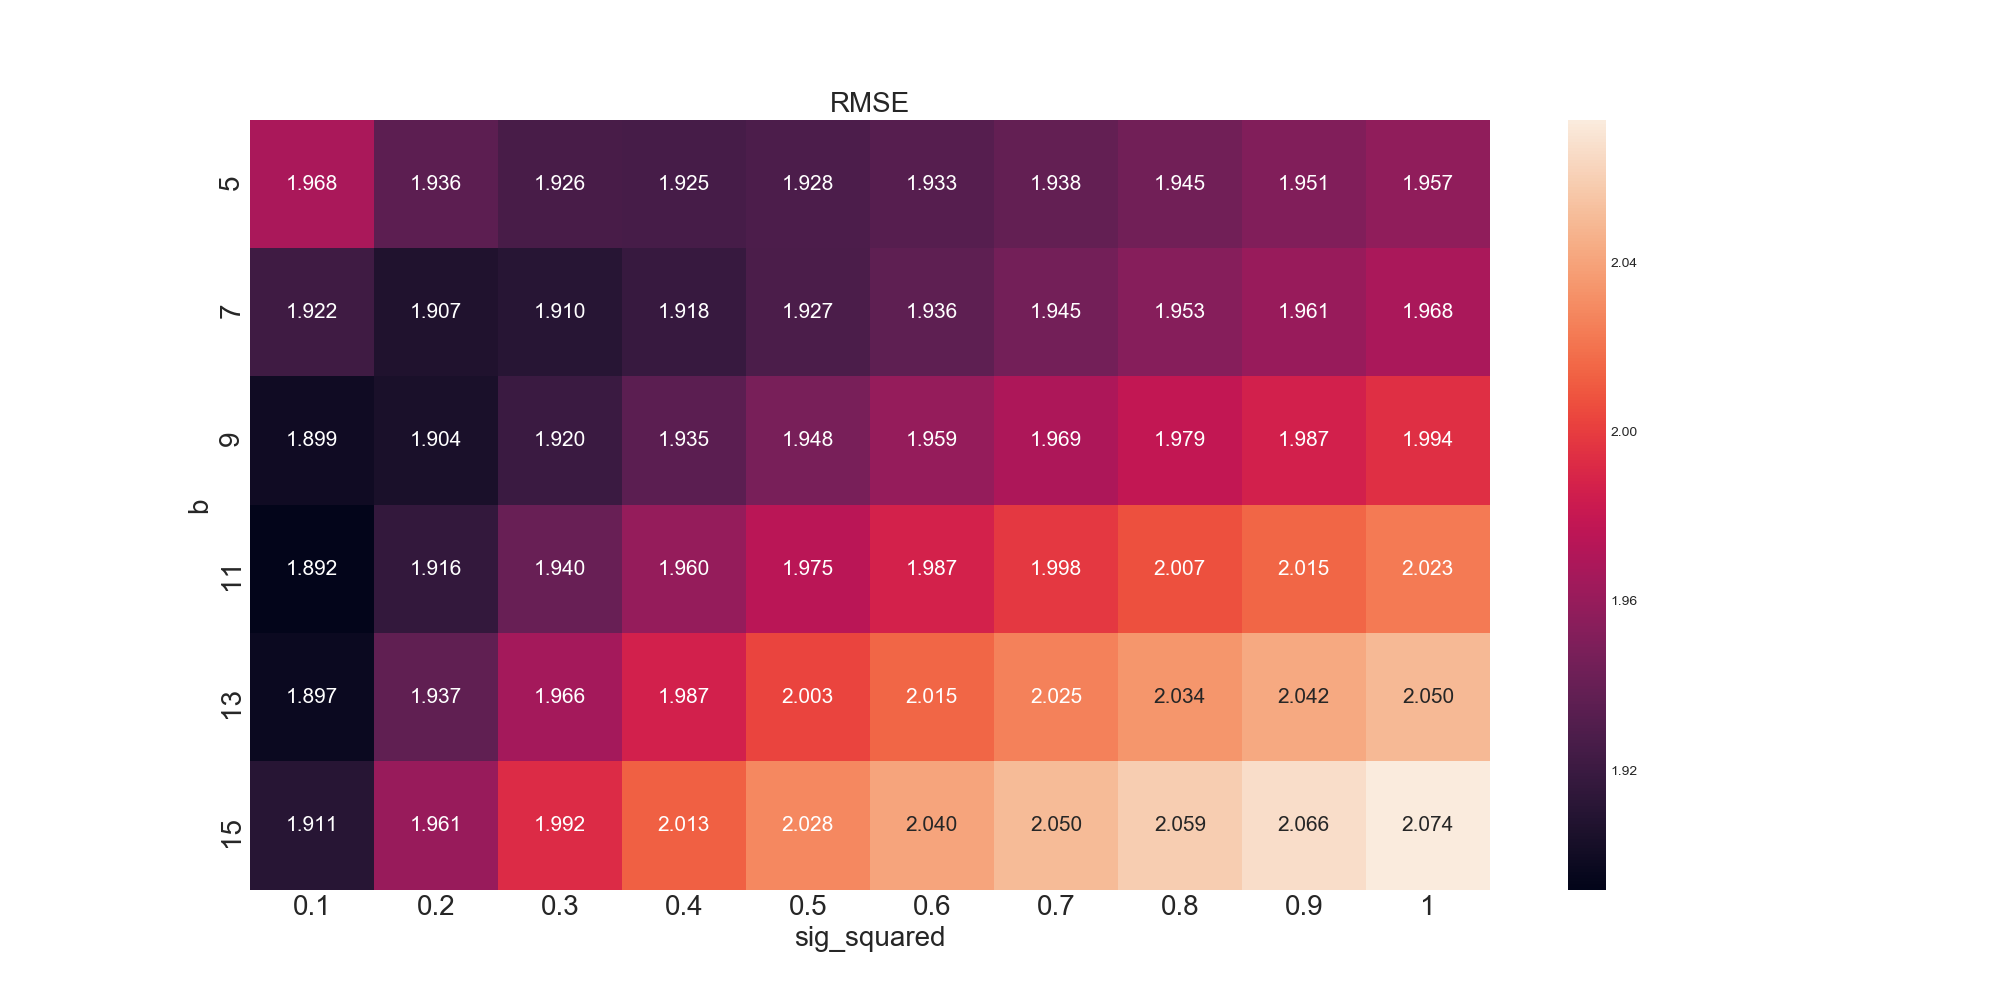
\includegraphics[width = \textwidth]{Homework_3_export/1b.png}
	\caption{Variation of RMSE for different values of b and $\sigma^2$}
\end{figure}

\section*{Problem 1(c)}

The least RMSE of 1.892 occurs for $\sigma^2 = 0.1$ and $b = 11$
\\
\\
The RMSE obtained on using a Linear Regression was 2.634. Therefore the lesat RMSE achieved from the Gaussian Process Regression is 28.17\% lower in comparision.
\\
\\
The RMSE obtained on using a Polynomial Ridge Regression of order 2 was 2.195. Therefore, the least RMSE achieved from Gaussian Process regression is 13.8\% lower in comparision.
\\
\\
One drawback of using Gaussian process regression over simple Linear regression is that it is a non-parametric machine learning algorithm. Therefore, there is no model/parameters stored after the training phase. This makes the prediction phase much slower in comparision to linear regression. Additionally, in terms of space, the linear regression needs to store a vector of length $d$, whereas the Gaussian process regression needs to store a Kernel of size $n^2$, which can be considerable for huge datasets.

\section*{Problem 1(d)}
\begin{figure}[h]
	\centering
	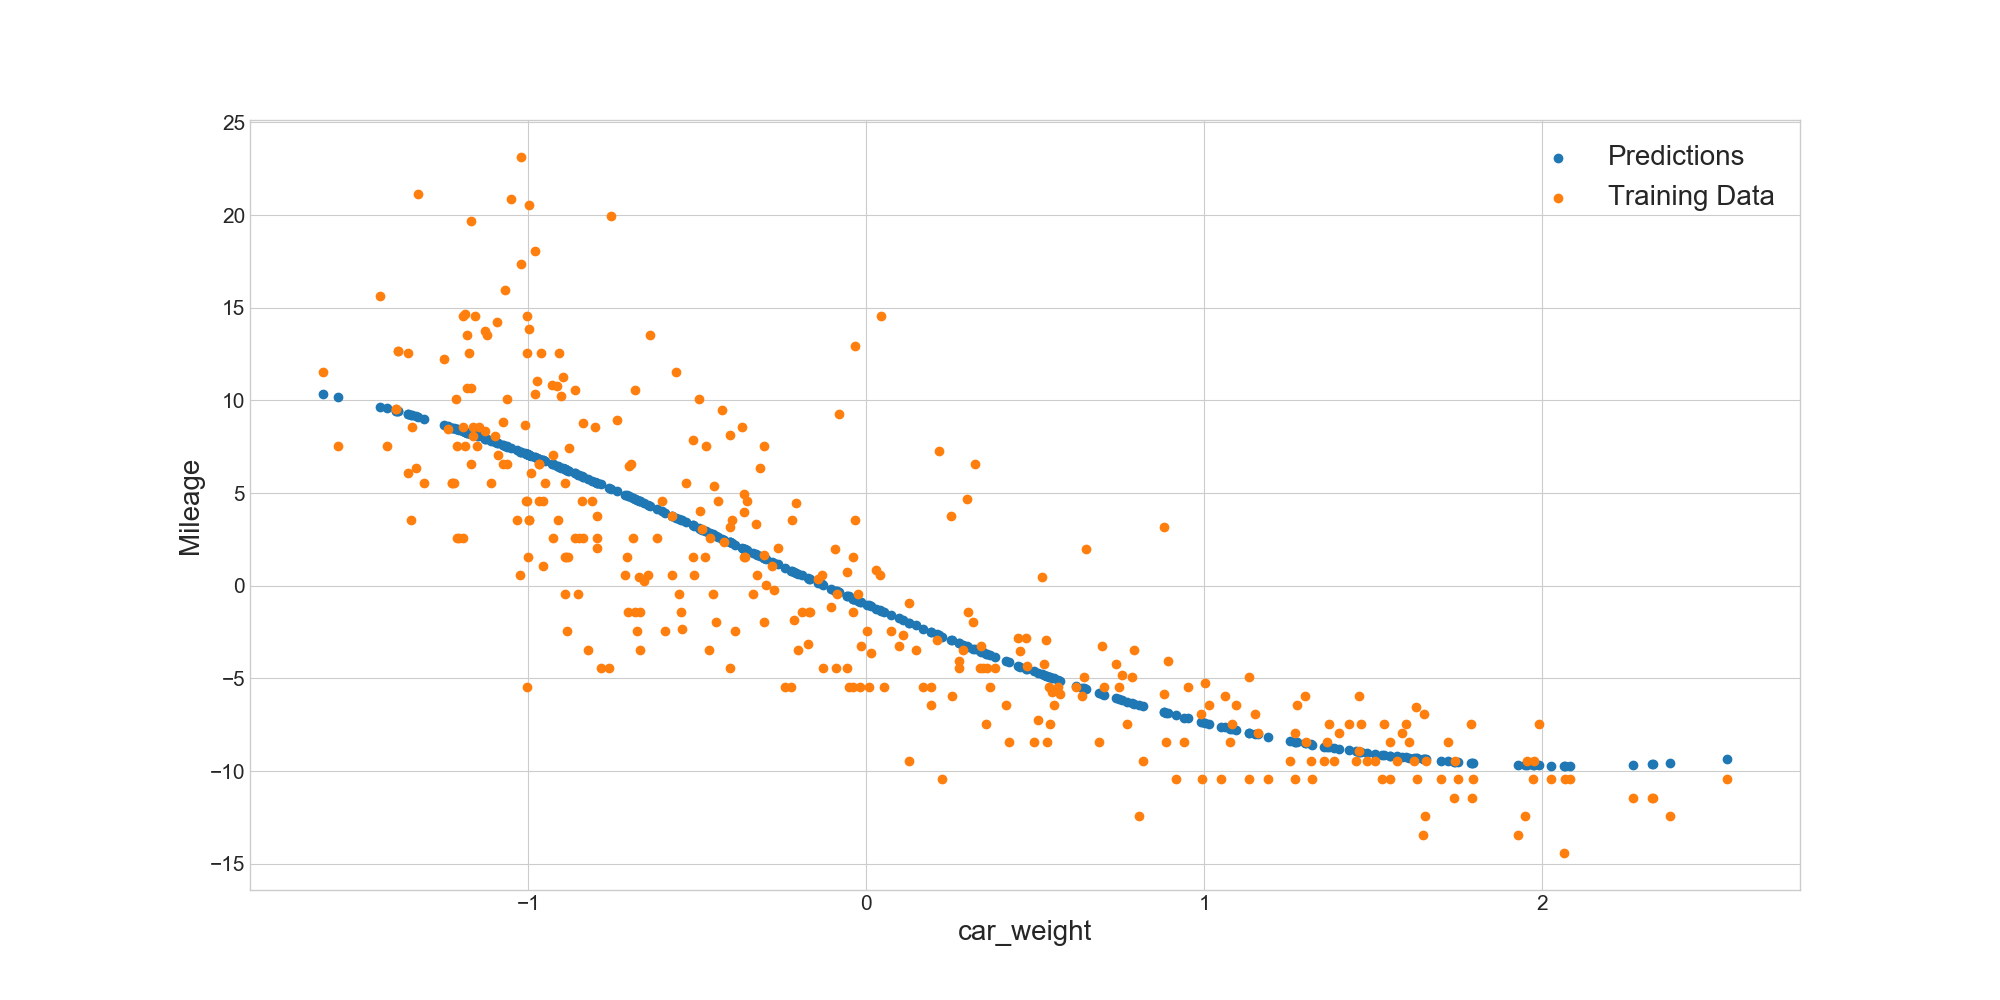
\includegraphics[width = \textwidth]{Homework_3_export/1d_new.png}
	\caption{Plot of Predicted values of y and Training labels vs. $x_4$}
\end{figure}

\section*{Problem 2(a)}

\begin{figure}[h]
	\centering
	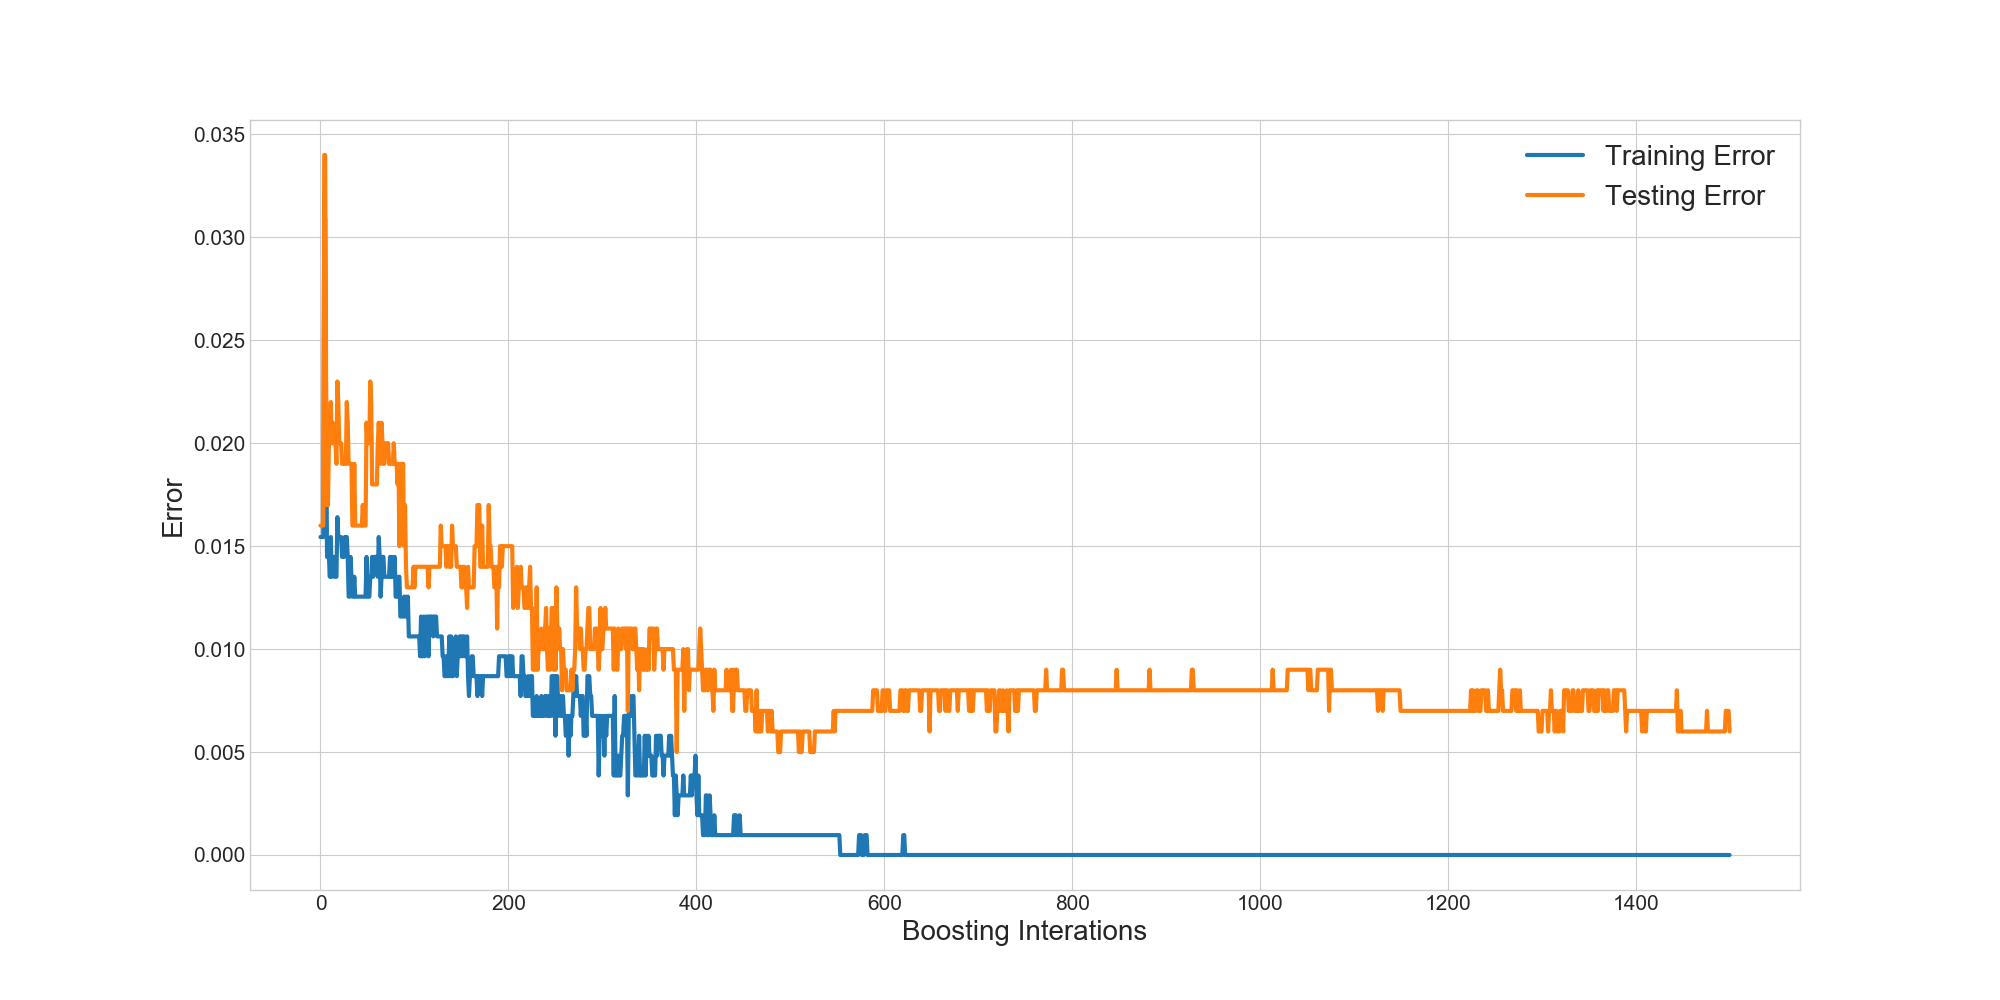
\includegraphics[width = \textwidth]{Homework_3_export/2a.png}
	\caption{Training and Testing Errors vs. Number of Classifiers Used}
\end{figure}

\textbf{Observation:} The training error is lower than the testing error as in the case of other machinel learning algorithms. 

\section*{Problem 2(b)}

\begin{figure}[h]
	\centering
	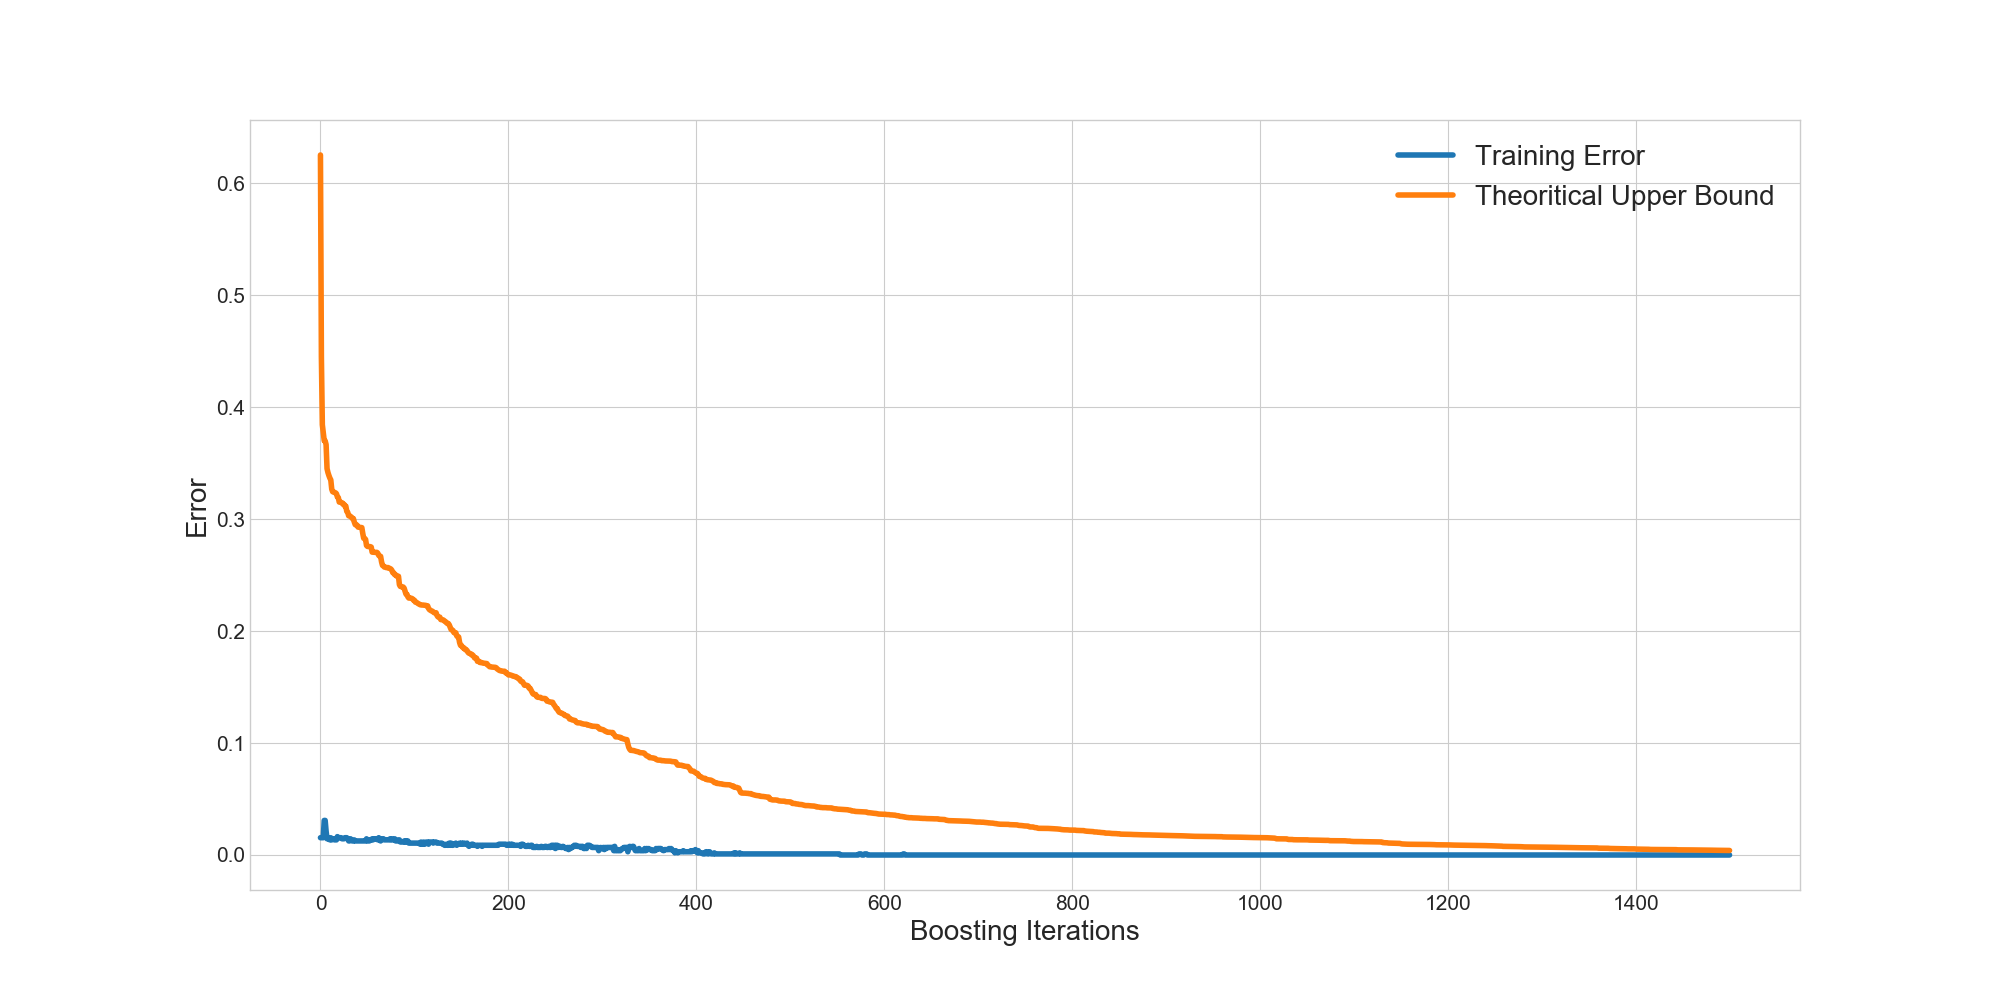
\includegraphics[width = \textwidth]{Homework_3_export/2b.png}
	\caption{Training Error and Theoritical Upper Bound vs. Number of Classifiers Used}
\end{figure}

\textbf{Observation:} The training error is lower than the theoretical upper bound, as it should be.

\section*{Problem 2(c)}

\begin{figure}[!h]
	\centering
	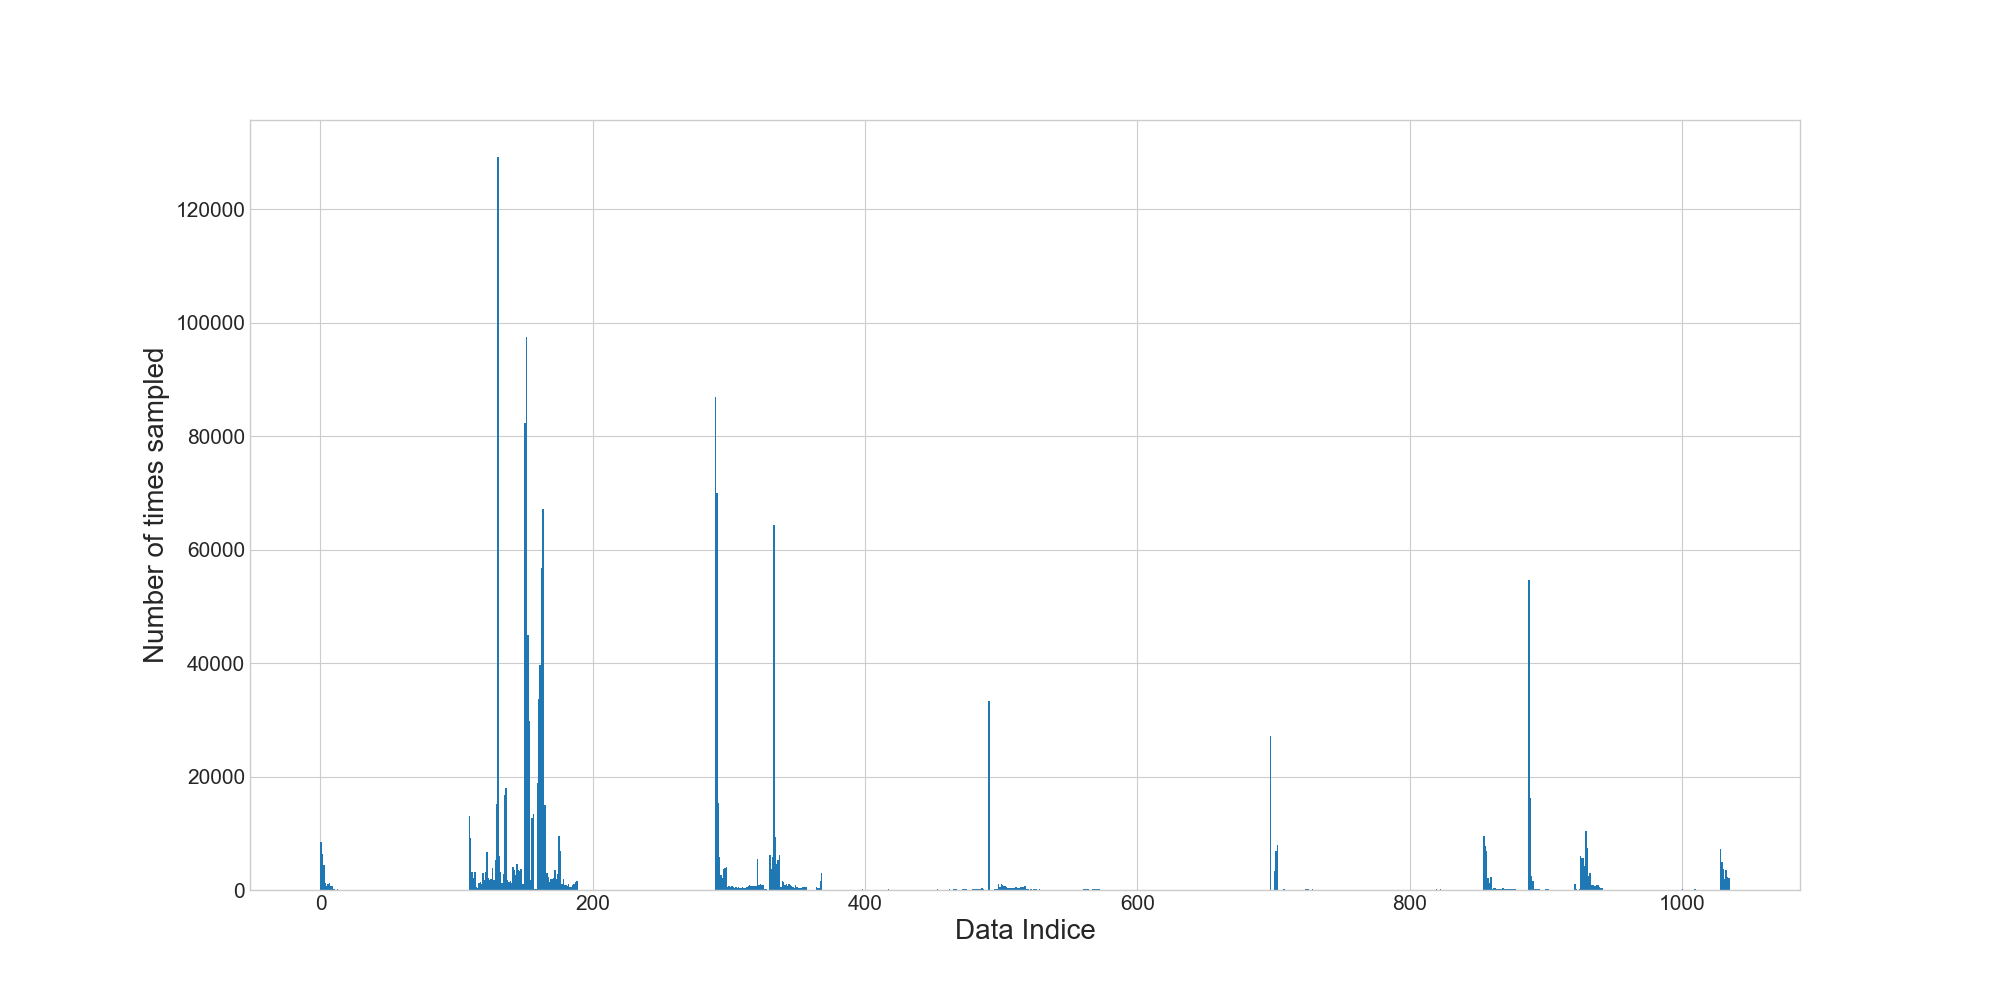
\includegraphics[width = 0.9\textwidth]{Homework_3_export/2c.png}
	\caption{Histogram of Sampling Frequency for each example in the training set}
\end{figure}

\begin{figure}[!h]
	\centering
	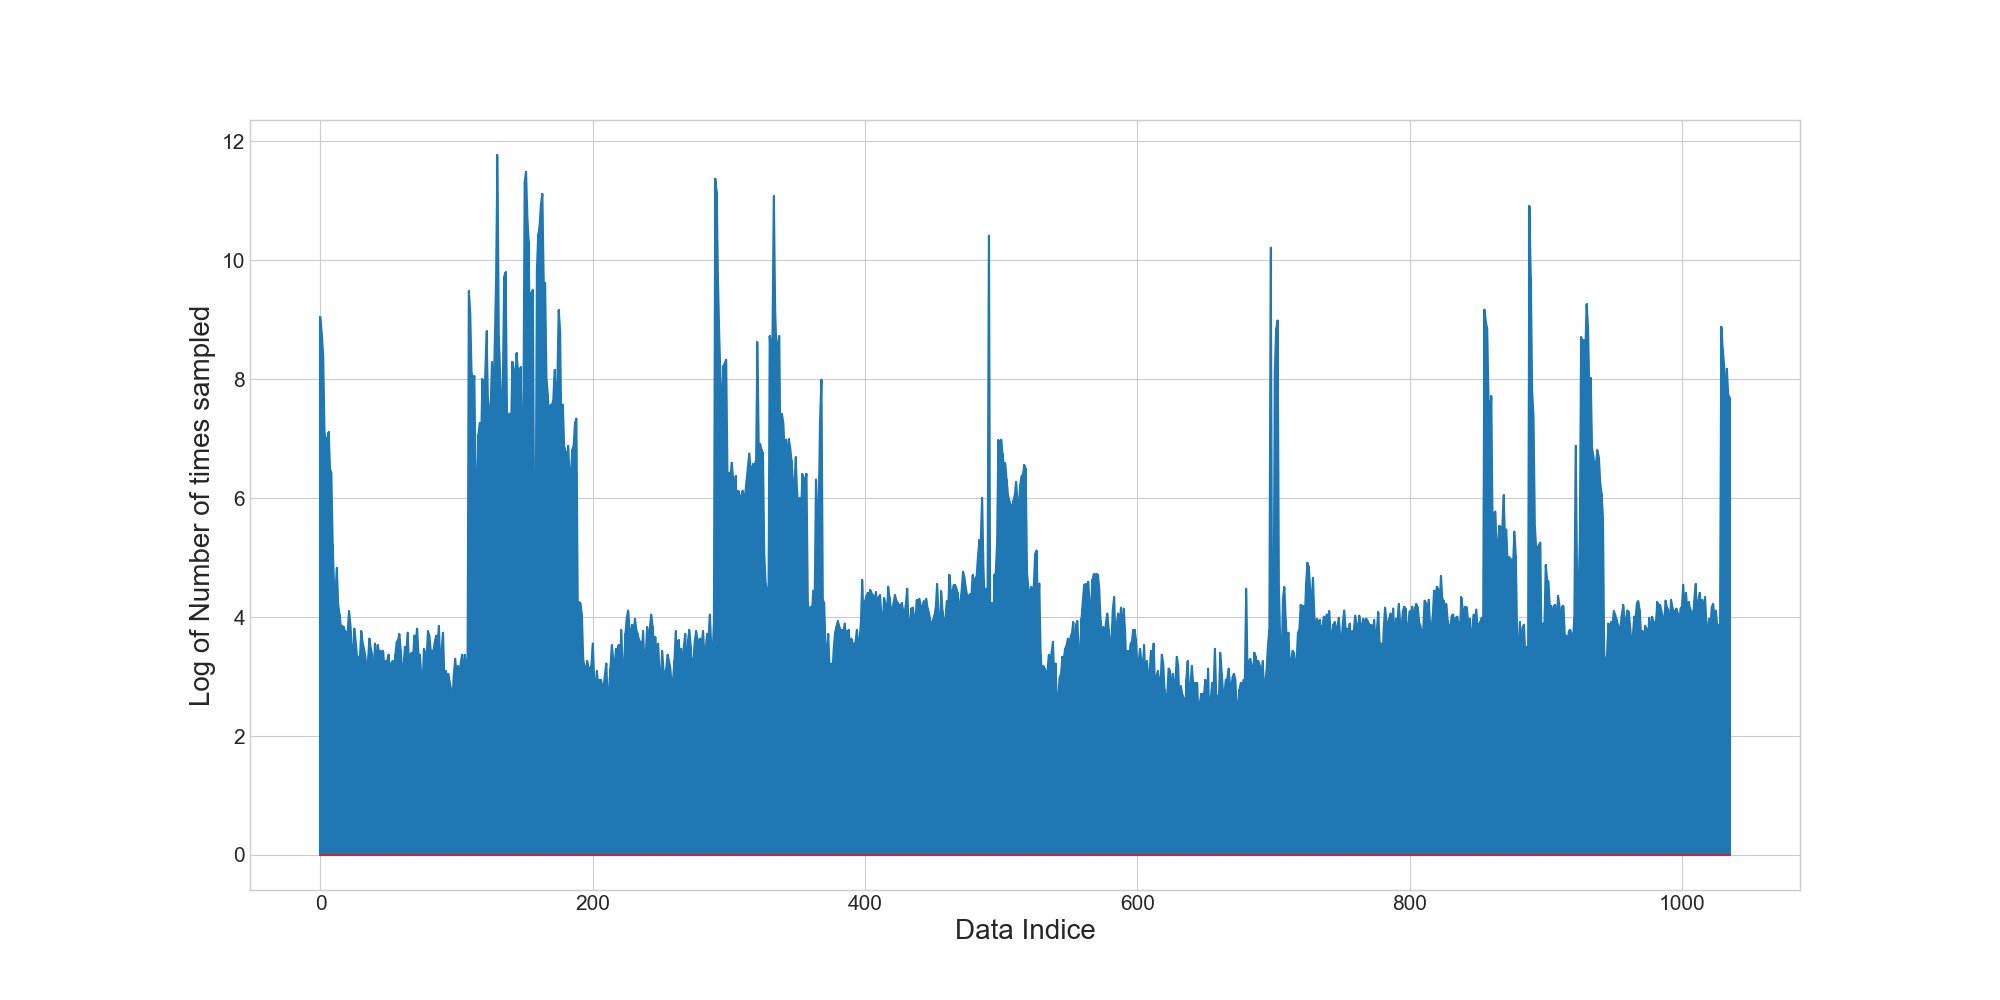
\includegraphics[width = 0.9\textwidth]{Homework_3_export/2c_log.png}
	\caption{Logarithmic Histogram of Sampling Frequency for each example in the training set}
\end{figure}

\textbf{Observation:} There are certain data points that are sampled more frequently than others. These could be assumed to be points that are near the decision boundary of the underlying data. The boosted classifier seems to sample these points more frequently to tweak its classification function.

\section*{Problem 2(d)}
\begin{figure}[!h]
	\centering
	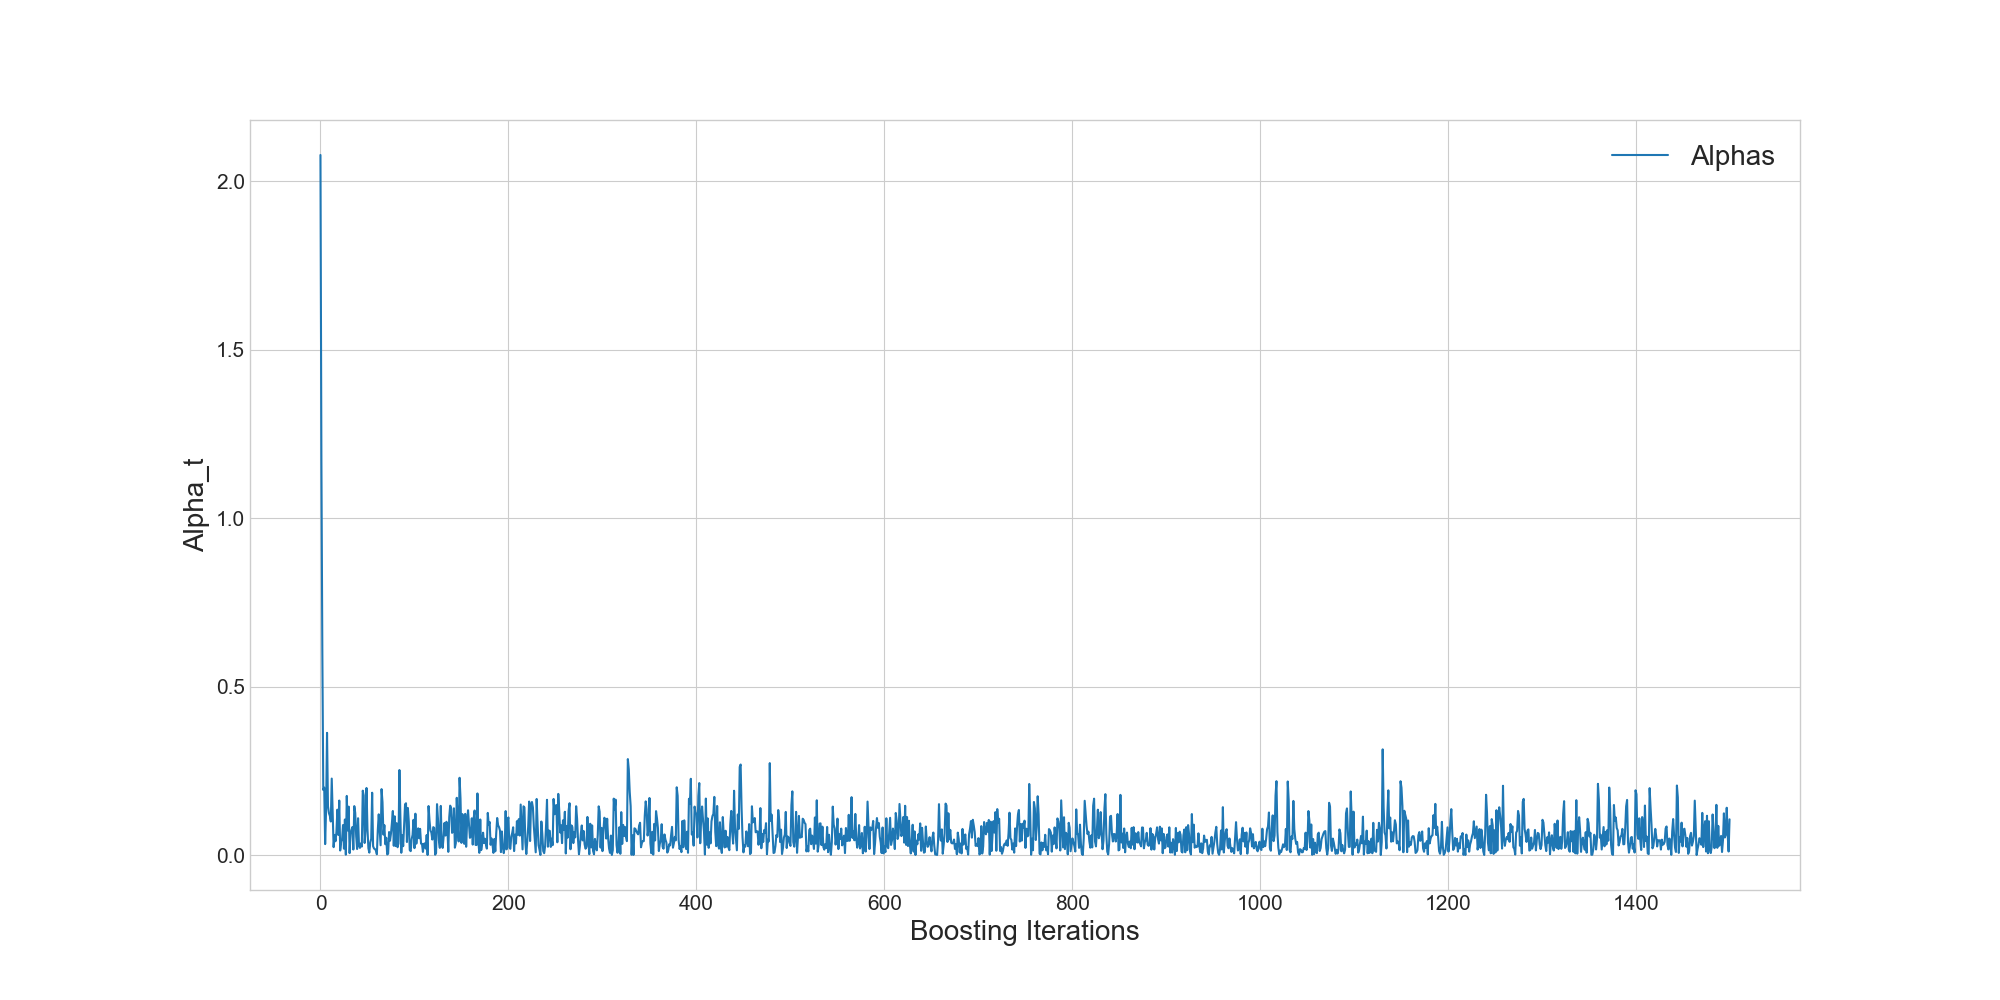
\includegraphics[width = \textwidth]{Homework_3_export/2da.png}
	\caption{$\alpha_t$ vs. No. of classifiers}
	\centering
	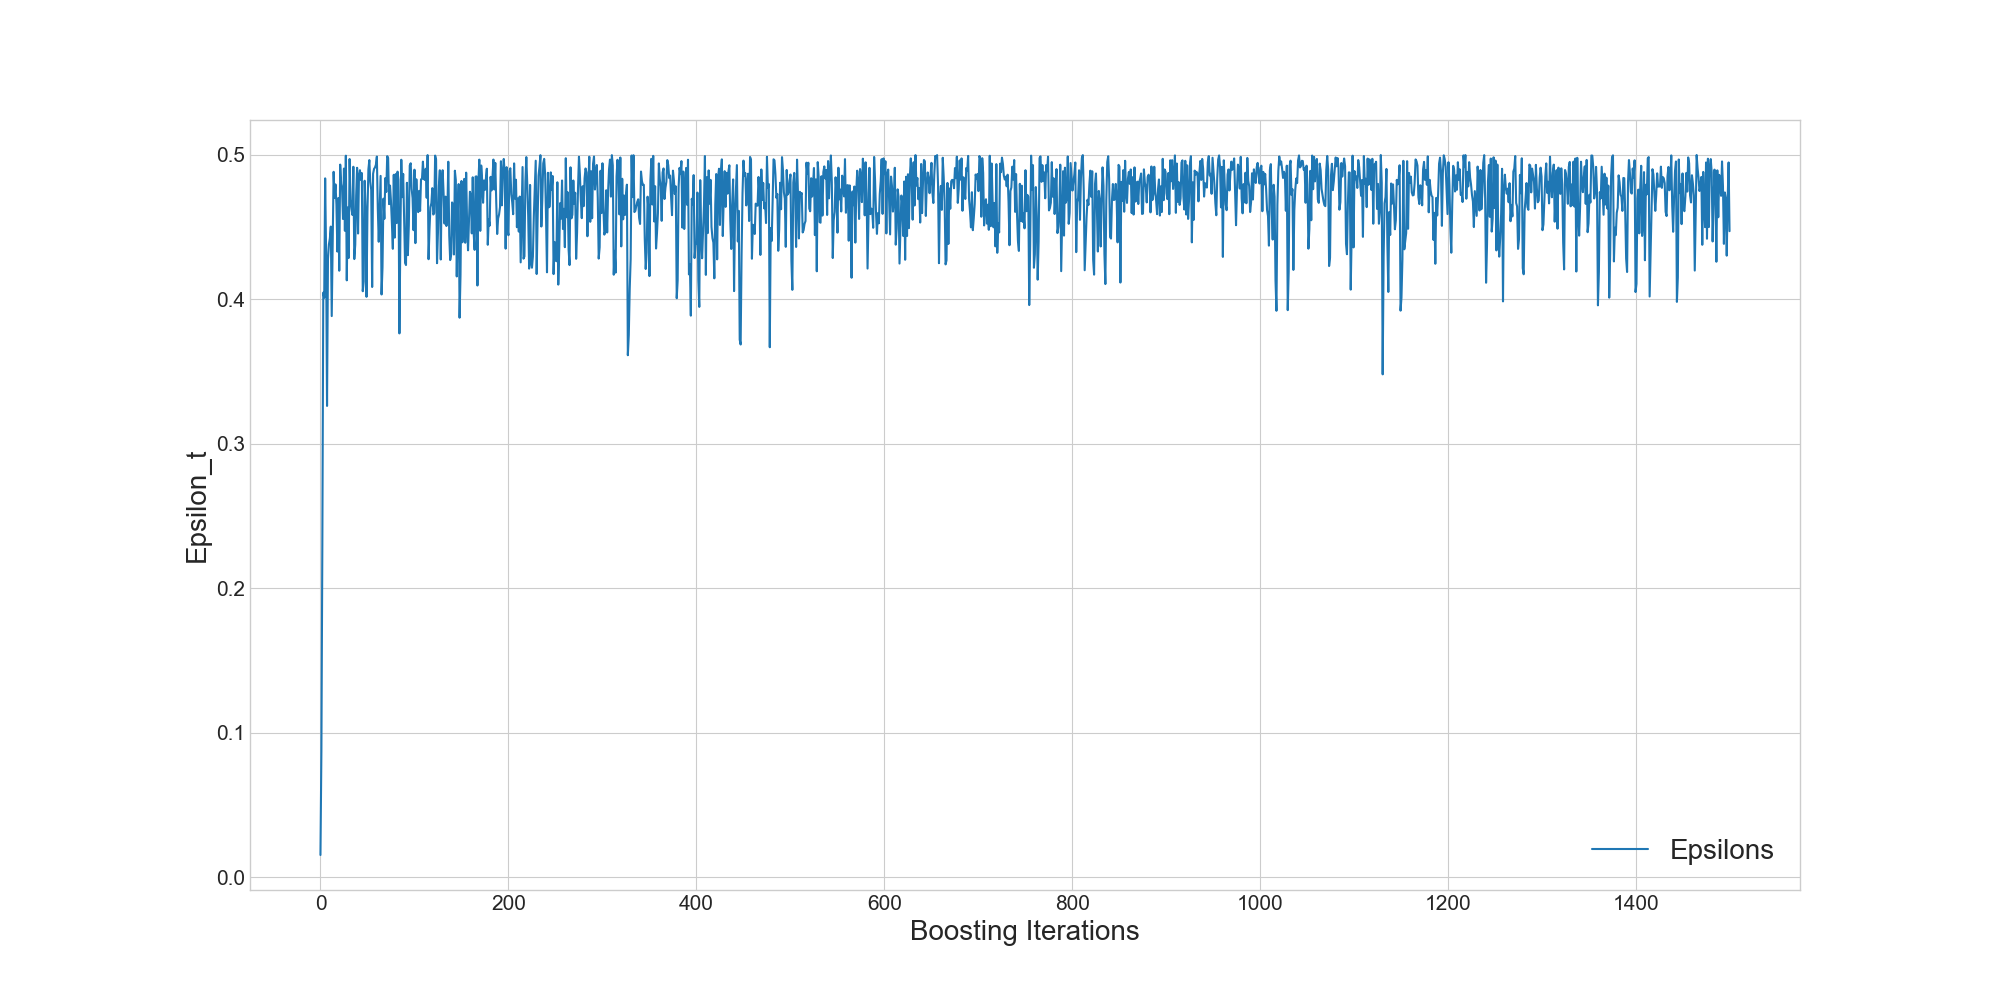
\includegraphics[width = \textwidth]{Homework_3_export/2de.png}
	\caption{$\epsilon_t$ vs. No. of classifiers}
\end{figure}

\textbf{Observation:} $\epsilon_t$ is mostly near and below 0.5. Consquently, $\alpha_t$, which is the weight for the $t^{th}$ classifier, is near and slightly above 0.

\end{document}
